\section{Experiments}\label{sec:experiments}

We investigated the impact of enforcing invariance on graph embeddings using three  datasets: Freebase15k-237\footnote{\tiny{\url{www.microsoft.com/en-us/download/details.aspx?id=52312}}}, MovieLens-1M\footnote{\tiny{\url{grouplens.org/datasets/movielens/1m/}}}, and an edge-prediction dataset derived from Reddit.\footnote{\tiny Using data from \url{ https://pushshift.io}, a previously existing dataset collected by Jason Baumgartner. The authors and their institutions were not involved in the data collection.} The dataset statistics are given in Table \ref{dataset_stats}. Our experimental setup closely mirrors that of \cite{madras2018learning} where we jointly train the main model with adversaries, but when testing invariance, we train a \textit{new} classifier (with the same capacity as the discriminator) to predict the senstive attributes from the learned embeddings.

The goal of our experiments was to answer three questions:
\begin{enumerate}[label={(\bf Q\arabic*)}, topsep=0pt, parsep=0pt, leftmargin=25pt, itemsep=2pt]
    \item \textbf{The invariance-accuracy tradeoff}. What is the tradeoff between enforcing invariance and accuracy on the main edge prediction task?
    \item \textbf{The impact of compositionality.} How does the performance of a compositional approach, which jointly enforces fairness over a set of sensitive attributes, compare to a more traditional model that only enforces fairness on a single attribute?
    \item \textbf{Invariance on unseen combinations.} In settings with many sensitive attributes, is our approach able to enforce invariance even on combinations of sensitive attributes that it never saw during training? 
\end{enumerate}
Throughout these experiments, we rely on two  baselines: First, we compare against baselines that do not include any invariance constraints, i.e., models with $\lambda=0$.
Second, we compare against a non-compositional adversarial approach where we separately train $K$ distinct encoders and $K$ distinct adversaries for each of the $K$ sensitive attributes in the data. 
This non-compositional adversary is essentially an extension of \citet{edwards2015censoring}'s approach to the graph embedding domain. 

\subsection{Setup and Datasets}

\begin{table*}[t]
\caption{Statistics for the three datasets, including the total number of nodes $(|\V|$) and number of nodes with sensitive attributes $|\T^*|$, the number of sensitive attributes and their types and the total number of edges in the graph.}
\label{datasetstats-table}
\begin{center}
\begin{small}
\begin{sc}
\begin{tabular}{lcccccr}
\toprule
Dataset & $|\V|$ & $|\T^*|$ &\multicolumn{1}{p{1.5cm}}{\centering \#Sensitive \\ Attributes} & Edges & \multicolumn{1}{p{1.5cm}}{\centering Binary \\ Attributes?} & \multicolumn{1}{p{1.5cm}}{\centering Multiclass \\ Attributes?} \\
\midrule
FB15k-237    & 14,940 & 14,940 & 3 & 168,618 &$\surd$ & $\times$ \\
MovieLens1M & 9,940& 6,040& 3& 1,000,209&$\surd$ &$\surd$\\
Reddit Comments    & 385,735 & 366,797& 10 &7,255,096 &$\surd$ & $\times$ \\
\bottomrule
\end{tabular}
\end{sc}
\end{small}
\end{center}
\vskip -0.1in
\label{dataset_stats}
\end{table*}



Before describing our experimental results, we first outline some important properties of the datasets we used, as well as the specific encoders and edge-prediction loss functions used.  

In all experiments, we used multi-layer perceptrons (MLPs) with leaky ReLU activation functions \cite{xu2015empirical} as the discriminators $D_k$ and filters $f_k$.
The Appendix contains details on the exact hyperparameters (e.g., number of layers and sizes) used for all the different experiments, as well as details on the training procedures (e.g., number of epochs and data splits).
Code to reproduce our results is available at:
\url{https://github.com/joeybose/Flexible-Fairness-Constraints}.

\subsubsection*{Freebase15k-237}
\vspace{-2mm}
Freebase 15k-237 is a standard benchmark used for knowledge base completion \cite{toutanova2015representing}.
In this work, we use Freebase 15k-237 as a semi-synthetic testbed to evaluate the impact of adversarial regularization. 
Taking the entity attribute labels from \citet{moon2017learning}, we used the $3$-most common attribute labels (e.g., /award/award\_nominee) as ``sensitive'' attributes.
The goal in this dataset is to perform the standard knowledge base completion task, while having the entity embeddings be invariant with respect to these ``sensitive'' attribute labels.
While synthetic, this dataset provides a useful reference point due to its popularity in the graph embedding literature. 

For our encoder and edge-prediction loss function, we follow \citet{ji2015knowledge}'s TransD approach, since we found this approach gave significant performance boosts compared to simpler models (e.g., TransE). 
In this model, the encoding of a node/entity depends on the edge relation being predicted, as well as on whether the entity is the head or tail in a relation (i.e., the edge direction matters).
In particular, the embedding of the head node (i.e., the source node) in an edge relation is given by:
\begin{equation}
    \enc(u, \langle u, r, v \rangle) = (\mb{r}_p\mb{u}_p^\top + \mb{I}^{d \times d})\mb{u},
\end{equation}
where $\mb{u}, \mb{u}_p, \mb{r}_p \in \mathbb{R}^d$ are trainable embedding parameters and $\mb{I}^{d\times d}$ is a $d$-dimensional identity matrix. 
The encoding function for the tail node is defined analogously. 
The score function for this approach is given by
\begin{align*}\label{eq:transd}
s(\langle u, r, v \rangle) = -\|\enc(u, \langle u, r, v \rangle) + &\mb{r} \\ - \enc(v, \langle u, r,& v \rangle)\|_2,
\end{align*}
where $\mb{r} \in \mathbb{R}^d$ is another trainable embedding parameter (one per relation). 
Finally, we use a standard max-margin loss with a single negative sample per positive edge:
\begin{equation}\label{eq:margin}
    L_{\textrm{edge}}(s(e), s(e^-)) = \max(0, 1 - s(e) + s(e)^-).
\end{equation}
\subsubsection*{Movielens-1M}
\vspace{-2mm}
Our second dataset is derived from the MovieLens-1M recommender system benchmark \cite{harper2016movielens}.
This is a standard recommender system benchmark, where the goal is to predict the rating that users assign movies.
However, unlike previous work, in our experiments we treat the user features (age, gender, and occupation) as sensitive attributes (rather than as additional feature information for the recommendation task). 
Following \citet{berg2017graph} we treat this recommendation task as an edge prediction problem between users and movies, viewing the different possible ratings as different edge relations. 

For this dataset we use a simple ``embedding-lookup'' encoder, where each user and movie is associated with a unique embedding vector in $\mathbb{R}^d$.
As a scoring function, we follow \citet{berg2017graph} and use a  log-likelihood approach:
\begin{equation*}
    s(\langle u, r, m \rangle) = \mb{z}_u^\top\mb{Q}_r\mb{z}_v-\log(\sum_{r' \in \mathcal{R}}\mb{z}_u^\top\mb{Q}_{r'}\mb{z}_v),
\end{equation*}
The relation matrices $\mb{Q}_r \in \mathbb{R}^{d \times d}$ are computed as:
\begin{equation*}
    \mb{Q}_r = a_{r, 1}\mb{P}_1 + a_{r,2}\mb{P}_2, 
\end{equation*}
where $a_{r, 1}, a_{r, 1} \in \R$ and $\mb{P}_1, \mb{P}_2 \in \R^{d \times d}$ are trainable parameters. 
In this case, the loss function is simply the negative of the log-likelihood score. 

\subsubsection*{Reddit}
\vspace{-2mm}
The final dataset we consider is based on the social media website Reddit---a popular, discussion-based website where users can post and comment on content in different topical communities, called ``subreddits''. 
For this dataset, we consider a traditional edge prediction task, where the goal is to predict interactions between users and subreddit communities. 

To construct the edge prediction task, we examined all comments from the month of November in $2017$, and we placed an edge between a user and a community if this user commented on that community at least once within this time period. 
We then took the $10$-core of this graph to remove low-degree nodes, which resulted in a graph with approximately $366$K users, $18$K communities, and $7$M edges.
Given this graph, the main task is to train an edge-prediction model on $90\%$ of the user-subreddit edges and then predict missing edges in a held-out test set of the remaining edges.  

Reddit is a pseudonymous website with no public user attributes.  
Thus, to define sensitive attributes, we treat certain subreddit nodes as {\em sensitive nodes}, and the sensitive attributes for users are whether or not they have an edge connecting to these sensitive nodes.
In other words, the fairness objective in this setting is to force the model to be invariant to whether or not a user commented on a particular community. 
To select the ``sensitive'' subreddit communities, we randomly sampled $10$ from the top-100 communities by degree.\footnote{We excluded the top-5 highest-degree outlying communities.} 
Note that this setting represents the extreme case where we want the model to be invariant with respect to the existence of particular edges in the input graph. 

As with MovieLens-1M, we use a simple ``embedding-lookup'' encoder. 
In this case, there is only a single relation type---indicating whether a Reddit user has commented on a ``subreddit'' community.
Thus, we employ a simple dot-product based scoring function,
   $s(\langle u, r, v \rangle) = \mb{z}_u^\top\mb{z}_v$,
and we use a max-margin loss as in Equation \eqref{eq:margin}. 

\subsection{Results}
We now address the core experimental questions (\textbf{Q1}-\textbf{Q3}). 

\begin{table*}[t]
\caption{Ability to predict sensitive attributes on the MovieLens data when using various embedding approaches. For gender attribute the score is AUC while for age and occupation attributes the score is micro averaged F1. The columns represent the different embedding approaches (e.g., with or without adversarial regularizatin) while the rows are the attribute being classified.}
\label{ml-table}
\begin{center}
\begin{small}
\begin{sc}
\begin{tabular}{lccccccr}
\toprule
MovieLens1M & \multicolumn{1}{p{1.5cm}}{\centering Baseline \\ No Adversary} & \multicolumn{1}{p{1.5cm}}{\centering Gender \\ Adversary} & \multicolumn{1}{p{1.5cm}}{\centering Age \\ Adversary} & \multicolumn{1}{p{1.5cm}}{\centering Occupation \\ Adversary}&\multicolumn{1}{p{1.5cm}}{\centering Comp. \\ Adversary} & \multicolumn{1}{p{1.5cm}}{\centering Majority \\ Classifier} & \multicolumn{1}{p{1.5cm}}{\centering Random \\ Classifier} \\
\midrule
Gender    & 0.712& 0.532& 0.541 & 0.551 & 0.511 & 0.5 & 0.5 \\
Age    & 0.412 & 0.341& 0.333 & 0.321 & 0.313 & 0.367 & 0.141\\
Occupation     & 0.146 & 0.141& 0.108 & 0.131 & 0.121 & 0.126 & 0.05 \\

\bottomrule
\end{tabular}
\end{sc}
\end{small}
\end{center}
\vskip -0.1in
\end{table*}


\begin{table}[t]
\caption{Ability to predict sensitive attributes on the Freebase15k-237 data when using various embedding approaches. AUC scores are reported, since all the sensitive attributes are binary. The mean rank on the main edge-prediction task is also reported.}
\label{fb15k-table}
\vskip 0.15in
\begin{center}
\begin{small}
\begin{sc}
\begin{tabular}{lcccr}
\toprule
FB15k-237 & \multicolumn{1}{p{1.5cm}}{\centering Baseline \\ No Adversary} & \multicolumn{1}{p{1.5cm}}{\centering Non \\ Comp. Adversary} & \multicolumn{1}{p{1.5cm}}{\centering Comp. \\ Adversary} \\
\midrule
Attribute 0    &0.97& 0.82& 0.77  \\
Attribute 1 & 0.99& 0.81& 0.79\\
Attribute 2   & 0.98&  0.81 & 0.81 \\
Mean Rank &285& 320 & 542 \\
\bottomrule
\end{tabular}
\end{sc}
\end{small}
\end{center}
\vskip -0.1in
\label{fb_exp}
\end{table}


\begin{figure}[t!]
    \centering
    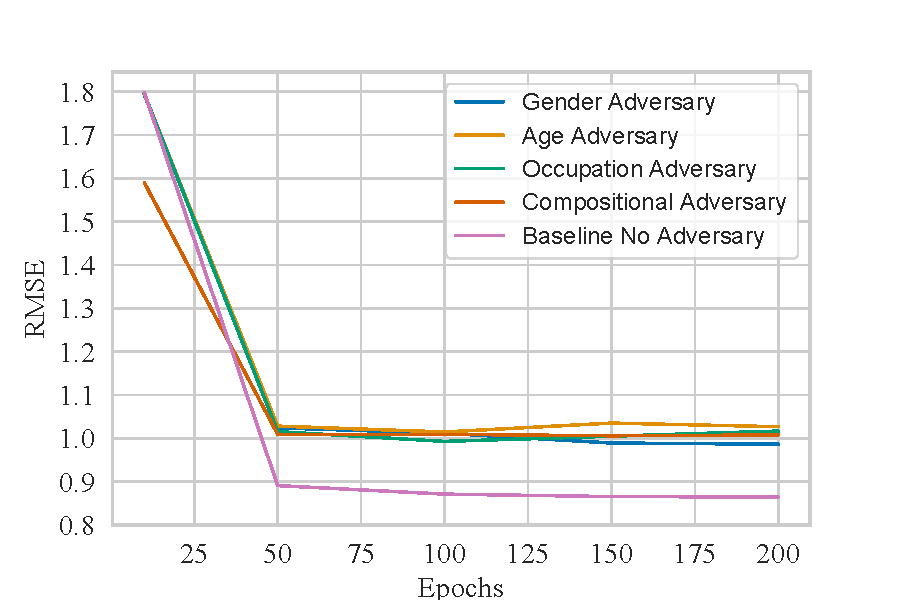
\includegraphics[width=0.9\linewidth]{plots/movielens1m_rmse.pdf}
    \vspace{-15pt}
    \caption{Performance on the edge prediction (i.e., recommendation) task on MovieLens, using RMSE as in \citet{berg2017graph}.}
    \label{fig:rmse}
    \vspace{-1mm}
\end{figure}
\begin{figure}[t!]
    \centering
    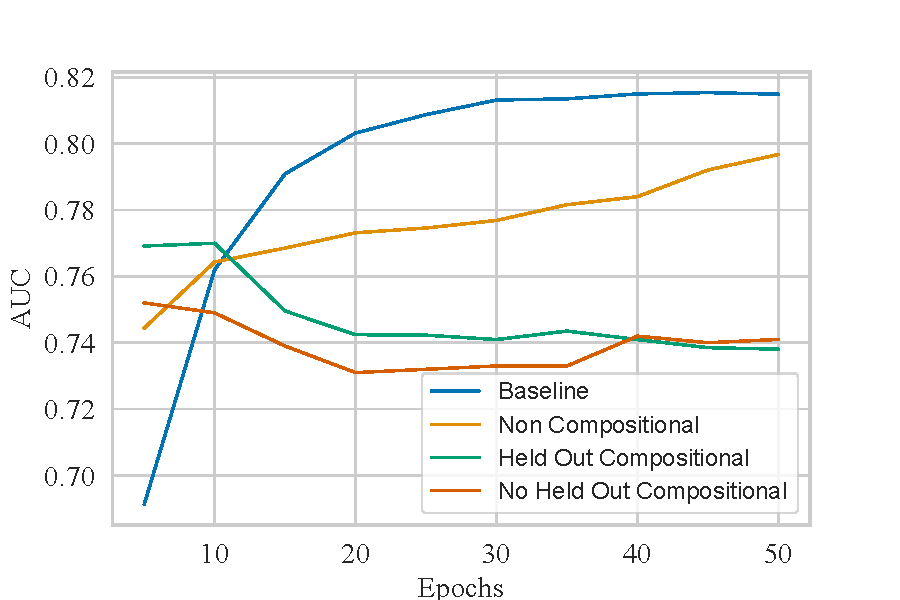
\includegraphics[width=0.9\linewidth]{plots/reddit_enc_auc.pdf}
       \vspace{-10pt}
    \caption{Performance on the edge prediction (i.e., recommendation) task on the Reddit data. Evaluation is using the AUC score, since there is only one edge/relation type.}
    \label{fig:reddit_enc_auc}
    \vspace{-2mm}
\end{figure}
\begin{figure}[t!]
    \centering
    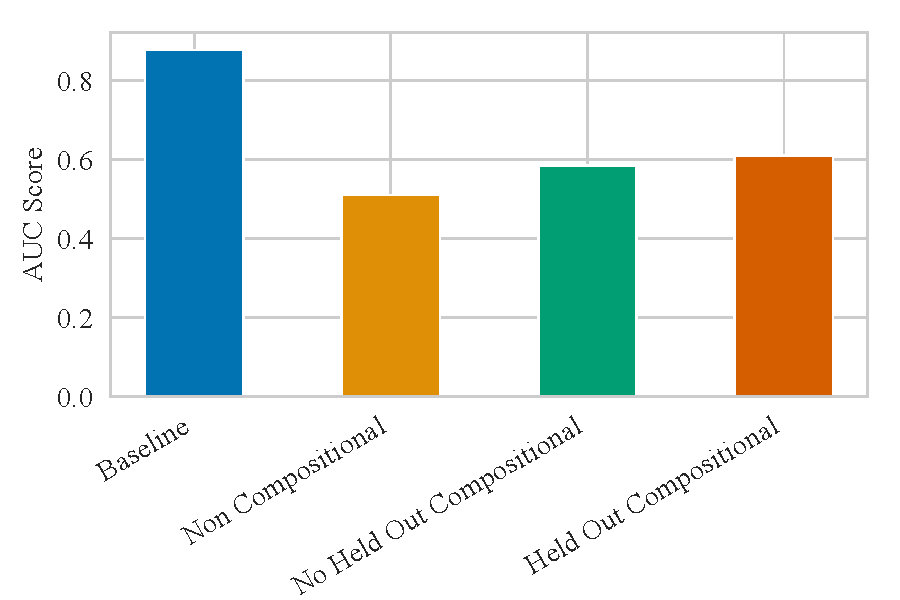
\includegraphics[width=0.9\linewidth]{plots/reddit_auc.pdf}
    \vspace{-15pt}
    \caption{Ability to predict sensitive attributes on the Reddit data when using various embedding approaches. Bar plots correspond to the average AUC across the $10$ binary sensitive attributes.}
    \label{fig:reddit_auc}
    \vspace{-2mm}
\end{figure}

\subsubsection*{Q1: The Invariance-Accuracy Tradeoff}

In order to quantify the extent to which the learned embeddings are invariant to the sensitive attributes (e.g., after adversarial training), we freeze the trained compositional encoder $\compenc$ and train an new MLP classifier to predict each sensitive attribute from the filtered embeddings (i.e., we train one new classifier per sensitive attribute).
We also evaluate the performance of these filtered embeddings on the original prediction tasks. 
In the best case, a newly trained MLP classifier should have random accuracy when attempting to predict the sensitive attributes from the filtered embeddings, but these embeddings should still provide strong performance on the main edge prediction task. Thus, for binary sensitive attributes, an ideal result is an AUC score of $0.5$ when attempting to predict the sensitive attributes from the learned embeddings. 

\begin{figure}
    \centering
    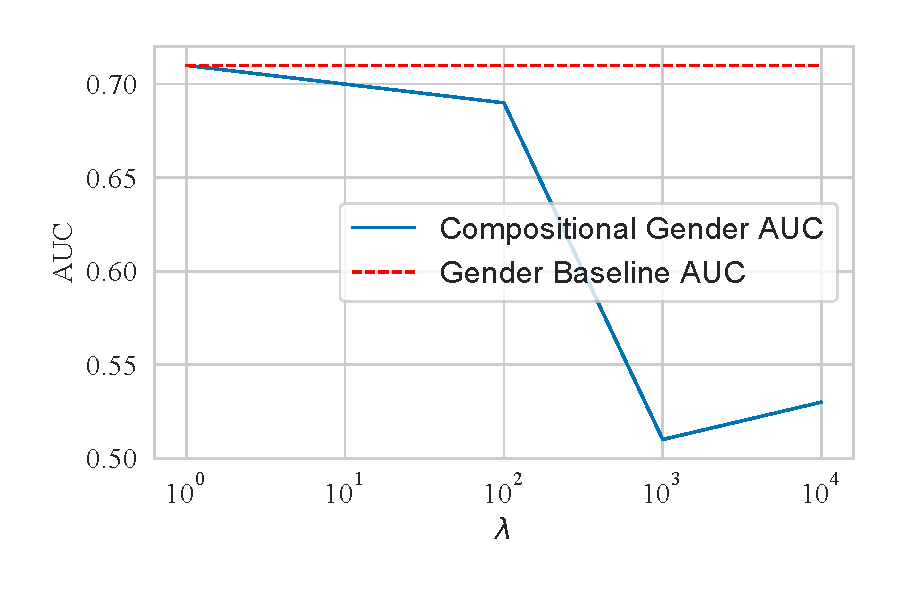
\includegraphics[width=0.9\linewidth]{plots/comp_gender_auc.pdf}
      \vspace{-15pt}
    \caption{Tradeoff of Gender AUC score on MovieLens1M for a compositional adversary versus different $\lambda$}
    \label{fig:comp_gender_auc}
\vspace{-2mm}
\end{figure}

Overall, we found that on the more realistic social recommendation datasets---i.e., the MovieLens-1M and Reddit datasets---our approach was able to achieve a reasonable tradeoff, with the near-complete removal of the sensitive information leading to a roughly 10\% relative error increase on the edge prediction tasks. In other words, on these two datasets the sensitive attributes were nearly impossible to predict from the filtered embeddings, while the accuracy on the main edge prediction task was roughly 10\% worse than a baseline approach that does not include the invariance constraints.
Table \ref{ml-table} and Figure \ref{fig:rmse} summarize these results for the MovieLens data, where we can see that the accuracy of classifying the sensitive attributes is on-par with a majority-vote classifier (Table \ref{ml-table}) while the RMSE degrades from $0.865$ to $1.01$ with the compositional adversary. Figures \ref{fig:comp_gender_auc} and \ref{fig:comp_gender_rmse} illustrate this tradeoff and show how the RMSE for the edge prediction task and ability to predict the sensitive attributes change as we vary the regularization strength, $\lambda$. As expected, increasing $\lambda$ does indeed produce more invariant embeddings but leads to higher RMSE values.
Figures \ref{fig:reddit_enc_auc} and \ref{fig:reddit_auc} similiarly summarize these results on Reddit. 

Interestingly, we found that on the Freebase15k-237 dataset it was not possible to completely remove the sensitive information without incurring a significant decrease in accuracy on the original edge prediction task. \cut{As we can see, for all values of $\lambda$ the ability to predict the sensitive attributes remains high (i.e., above 0.75 AUC) while the mean rank begins to degrade with higher $\lambda$ values.}
This result is not entirely surprising, since for this dataset the ``sensitive'' attributes were synthetically constructed from entity type annotations, which are presumably very relevant to the main edge/relation prediction task. 
However, it is an interesting point of reference that demonstrates the potential limitations of removing sensitive information from learned graph embeddings.  

\begin{figure}
    \centering
    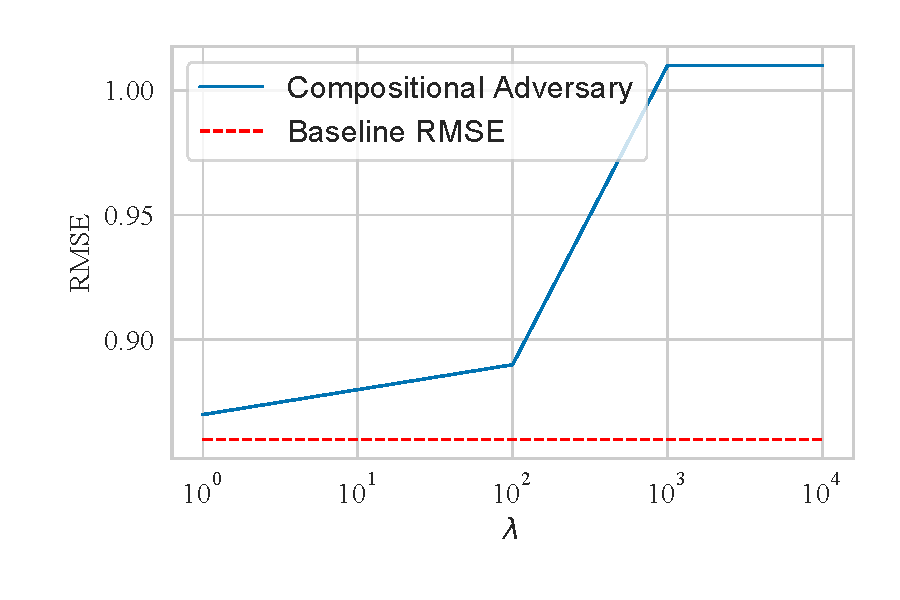
\includegraphics[width=0.9\linewidth]{plots/comp_gender_rmse.pdf}
      \vspace{-10pt}
    \caption{RMSE on MoveLens1M with various $\lambda$.}
    \label{fig:comp_gender_rmse}
\end{figure}

\subsubsection*{Q2: The Impact of Compositionality}

In all our experiments, we observed that our compositional approach performed favorably compared to an approach that individually enforced fairness on each individual attribute. In fact, on the MovieLens-1M data (and the synthetic Freebase15k-237 data), the compostionally trained adversary {\em outperformed} the individually trained adversaries in terms of removing information about the sensitive attributes (Table \ref{ml-table}). 
In other words, training a model to jointly remove information about the sensitive attributes using the compositional encoder (Equation \ref{eq:compenc}) removed more information about the sensitive attributes than training separate adversarially regularized embedding models for each sensitive attribute.
This result is not entirely surprising, as it essentially indicates that the different sensitive attributes (age, gender, and occupation) are correlated in this dataset. 
Nonetheless, it is a positive result indicating that the extra flexibility afforded by the compositional approach does not necessarily lead to a decrease in performance. 
That said, on the Reddit data we observed the opposite trend and found that the compositional approach performed worse in terms of its ability to remove information about the sensitive attributes (Figure \ref{fig:reddit_auc}) as well as a small drop on the performance of the main edge prediction task (Figure \ref{fig:reddit_enc_auc}). 

\subsubsection*{Q3: Invariance on Unseen Combinations}\label{subsubsec:comp_generalizability}

One of the key benefits of the compositional encoder is that it can flexibly generate embeddings that are invariant to any subset of $S \subseteq \{1, ..., K\}$ of the sensitive attributes in a domain. 
In other words, at inference time, it is possible to generate $2^K$ distinct embeddings for an individual node, depending on the exact set of invariance constraints. 
However, given this combinatorially large output space, a natural question is whether this approach performs well when generalizing to unseen combinations of sensitive attributes.

We tested this phenomenon on the Reddit dataset, since it has the largest number of sensitive attributes (10, compared to 3 sensitive attributes for the other two datasets). 
During training we held out $10\%$ of the combinations of sensitive attributes, and we then evaluated the model's ability to enforce invariance on this held-out set.
As we can see in Figure \ref{fig:reddit_auc}, the performance drop for the held-out combinations is very small ($0.025$), indicating that our compositional approach is capable of effectively generalizing to unseen combinations. 
The Appendix contains further results demonstrating how this trends scales gracefully when we increase the number of sensitive attributes from 10 to 50. 

\subsubsection*{Quantifying Bias}
In all of the above results, we used the ability to classify the sensitive attributes as a proxy for bias being contained within the embeddings.
While this is a standard approach, e.g., see \citet{edwards2015censoring}, and an intuitive method for evaluating representational invariance---a natural question is whether the adversarial regularization also decreases bias in the edge prediction tasks. 
Ideally, after filtering the embeddings, we would have that the edge predictions themselves are not biased according to the sensitive attributes.

To quantify this issue, we computed a ``prediction bias'' score for the MovieLens1M dataset: For each movie, we computed the absolute difference between the average rating predicted for each possible value of a sensitive attribute and we then averaged these scores over all movies. 
Thus, for example, the bias score for gender corresponds to the average absolute difference in predicted ratings for male vs.\@ female users, across all movies. From the perspective of fairness our adversary imposes a soft demographic parity constraint on the main task. A reduction in prediction bias across the different subgroups \cut{for a sensitive attribute} represents an empirical measure of achieving demographic parity.
Figure \ref{fig:pred_bias} highlights these results, which show that adversarial regularization does indeed drastically reduce prediction bias. Interestingly, using a compositional adversary works better than a single adversary for a specific sensitive attribute which we hypothesize is due to correlation between sensitive attributes.

\begin{figure}
    \centering
    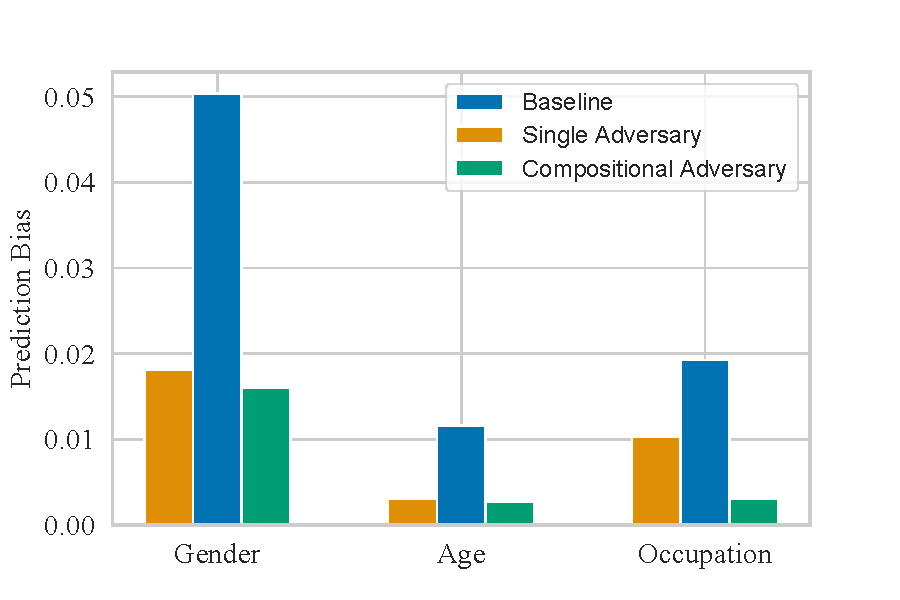
\includegraphics[width=0.9\linewidth]{plots/movielens1m_pred_bias.pdf}
    \vspace{-15pt}
    \caption{Prediction Bias for different Sensitive Attributes under three settings in MovieLens1M.}
    \label{fig:pred_bias}
    \vspace{-2.5mm}
\end{figure}








